
%%%%%%
%
% $Autor: Wings $
% $Datum: 2020-01-18 11:15:45Z $
% $Pfad: WuSt/Skript/Produktspezifikation/powerpoint/ImageProcessing.tex $
% $Version: 4620 $
%
%%%%%%

\chapter{Deployment}
\section{Test}

\subsection{General Tests}

All the Arduino boards need power to operate, either it comes from the USB connection with Laptop, Ac power adapter, Battery or a regulated power supply. The most easiest way to operate arduino board is USB connection with laptop, normally these boards need 5V direct current (DC) to operate. Arduino Nano 33 BLE sense also need these types of power sources for funcnality, when applying one of the above mention power source the green LED glows as shown in the figure \ref{fig:Test}, it shows the sign of Arduino board working.

\begin{figure}[htbp]
	\centering
	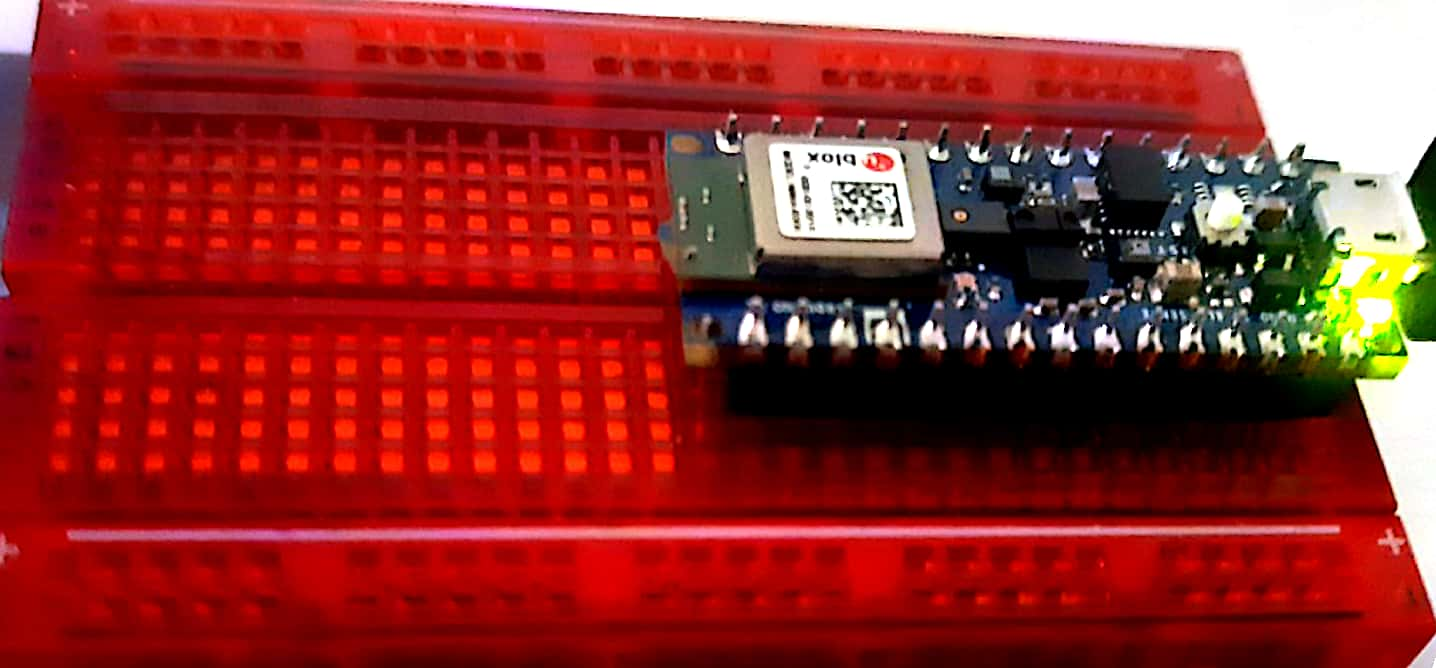
\includegraphics[width=6.5cm]{Images/Arduino/Test-1}
	\caption{Power On Arduino Nano 33 BLE Sense}
	\label{fig:Test}
\end{figure}

\subsection{Test with Bluetooth Module Connection}

The same procedure we need to follow for making the successful bleutooth coonection, the one we follow for on-board sensors. Below figure \ref{fig:testsoftware-fur-bluetooth} shows the ArduinoBLE library in the example section of Arduino IDE.

\begin{figure}[h]
	\centering
	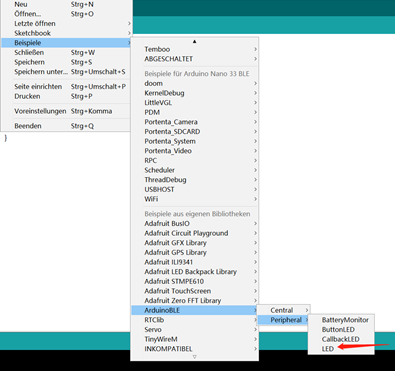
\includegraphics[width=0.7\linewidth]{Images/Arduino/TestsoftwareBluetooth}
	\caption{Bluetooth Connection}
	\label{fig:testsoftware-fur-bluetooth}
\end{figure}

Bluetooth wireless technology allows us to share the data, the voice, the music, the video, and a lot of information between paired devices, It is built into many products, from mobile phones, cars to medical devices and computers. It has lower power consumption. It is easily upgradeable. It has range better than Infrared communication. Bluetooth is used for voice and data transfer, we can communicate by recieving and sending the data with other bluetooth connected devices. It is also possible to output a value on the phone side or also on the laptop by making the proper pairing. 



\section{ML Pipeline}
\subsection{Using of TensorFlow}
TensorFlow: General, uses, user manual  

\subsection{Using Of TensorFlow Lite}
\subsection{Using Of TensorFlow Micro}
\subsection{Creating the Application with the Arduino IDE}
\section{Application "Recognizing Gait Patterns}
\subsection{Installation}
\subsection{Configuration}
\subsection{Tests}
\subsection{In the Field}
\section{Monitoring}
\section{Questions/To dos/ Conclusion}
\section{Appendix}
\subsection{Material List}
\subsection{Data sheets}